\documentclass[twocolumn,10pt]{asme2e}
\special{papersize=8.5in,11in}

\usepackage{graphicx}
\usepackage{amsmath}

\confshortname{IMECE 2014}
\conffullname{ASME 2014 International Mechanical Engineering Congress \& Exposition}
\confdate{14-20}
\confmonth{November}
\confyear{2014}
\confcity{Montreal}
\confcountry{Canada}

\papernum{IMECE2014-40187}

\title{TOWARDS A SUPERMILEAGE AUTONOMOUS VEHICLE}

\author{ Pedro Aguiar\\
    {\tensfb Paulina Ferretiz \thanks{Address all correspondence to this author.}}\\
    {\tensfb C\'{e}sar Hern\'{a}ndez} \\   
    {\tensfb Jorge Lozoya-Santos} \\   
    \affiliation{
    Engineering Department\\
    University of Monterrey\\
    San Pedro Garza Garcia, NL, 66238\\
    Mexico\\
    \scriptsize \{pedro.aguiar, paulina.ferretiz, cesar.hernandezr, jorge.lozoya\}@udem.edu
    }
}

\author{S\'{e}bastien Varrier\\
    \affiliation{
LCIS\\
Grenoble INP / ESISAR\\
Valence, 26902\\
France\\
\small sebastien.varrier@esisar.grenoble-inp.fr\\
}
}

\begin{document}

\maketitle    

%%%%%%%%%%%%%%%%%%%%%%%%%%%%%%%%%%%%%%%%%%%%%%%%%%%%%%%%%%%%%%%%%%%%%%
\begin{abstract}
{\it The project consists on the mechanical and electronic instrumentation
of an existing vehicle (built at Universidad de Monterrey for the SAE
Supermileage Competition) to be able to control its steering, braking and
throttle systems ``by wire". Insight to the stages of turning the vehicle into
an autonomous one is presented. This includes identification of the current
mechanical properties, chosing adequate components and the use of a simulation
to allow early work on the software involving cameras and motors to provide
autonomy to the vehicle. Using software in the loop methodology
mathematical models of the dynamics of the vehicle are run in Simulink
and update the position and orientation of the 3D model of the vehicle
in V-REP---a robot simulator.}

\noindent{\bf Keywords:} {\it Control engineering, vehicle dynamics, by-wire, autonomous vehicles, software in the loop, v-rep, simulator. }
\end{abstract}

%%%%%%%%%%%%%%%%%%%%%%%%%%%%%%%%%%%%%%%%%%%%%%%%%%%%%%%%%%%%%%%%%%%%%%
\section*{INTRODUCTION}

When a non-autonomous machine is converted into an autonomous one the
interfacing of the mechanical, human-actuated, components to an electrical
network is a key task. This is commonly known as ``by-wire" technology (e.g.
steer-by-wire) and makes it possible for a controller implemented in a
digital processor to operate the machine. In order for the controller to
do anything useful with its now-operable machine it usually needs sensors
to get data (classically human-gathered) from its environment.

The electrically interfaced mechanical components are accurately driven by
processing units that gather information from the electronic hardware and
apply a fitting logic to compute and generate a control signal.

\begin{figure}
\begin{center}
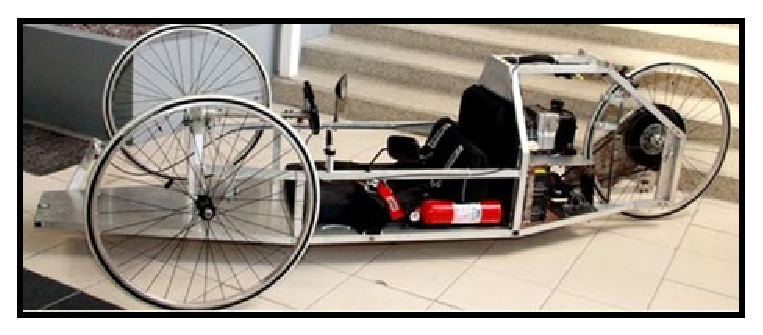
\includegraphics[width=11cm, natwidth=466, natheight=192]{figs/fig_vas_real.eps}
\caption{Initial state of the target vehicle}
\label{figs/fig_vas_real}
\end{center}
\end{figure}

Additionally to enabling automation, ``by-wire" technology allows for the
replacement and/or removal of mechanisms used to transmit force or movement
from one point to another in classic, mechanical machines. This can reduce
weight, increase available space and allow for more flexibility.

The merits of steer-by-wire technology in terms of space and fuel efficiency,
and the safety they offer over traditional mechanical systems have been
highlighted in the past \cite{fahami, qiang}. Research on realistic driving
feeling through feedback \cite{nguyen}, power assisted \cite{murugan} and
fully autonomous \cite{smith, silva} steering systems has been done. Mathematical
models of steer-by-wire systems and their control have been published
\cite{chang, fahami}. Testing and simulation of such work is being done
through software \cite{fahami} and hardware-in-the-loop simulations
methodologies\cite{park}. All this work on vehicle's dynamics provides
the mechanical foundation for the development of an autonomous vehicle,
which also relies on areas such as artificial intelligence and control
engineering.

The objective of this publication is to present, generally, the work
that is being done to convert a fully functional combustion engine
vehicle into an autonomous one, removing the mechanical interfaces
---pedal, steering wheel, brake lever---to the vehicle. Equations describing the
dynamics of a vehicle are used to move a 3D model of the vehicle in
a virtual environment. This movement, which is controlled by the
input current of a motor in a steer-by-wire system, allows testing
of computer vision algorithms. That is, a program modify the value
reresenting the input current to the modeled steering motor in function of
what the simulated cameras capture from the virtual environment.

This article contains the following sections: The first is about
the supermileage autonomous vehicle, the target vehicle is introduced,
the electronic architecture is presented, the mechanism designed for
the steer-by-wire system of the vehicle and the much simpler
brake and throttle-by-wire instrumentation are exposed; at the third section
the interaction of a mathematical model used to approximate the vehicle's
dynamics, its assembly using Simulink and a simulated environment used
to form a development and testing platform for computer vision and control
algorithms is discussed; finally, fourth section states the results,
conclusions and possible further work.

%%%%%%%%%%%%%%%%%%%%%%%%%%%%%%%%%%%%%%%%%%%%%%%%%%%%%%%%%%%%%%%%%%%%%%
\section*{SUPERMILEAGE AUTONOMOUS VEHICLE}

\subsection*{Target Vehicle}
The vehicle is a combustion engine powered, three-wheeler made of
aluminium. It has bicycle wheels, chain transmission and a V-brake.
The steering, braking and throttling systems are actuated by the
driver through a steering wheel, a brake lever (such as the ones commonly
found on bicycles) and a pedal, respectively. An image of the
vehicle is shown in figure~\ref{figs/fig_vas_real}. Some of the
parameters of the vehicle are shown in table~\ref{vas_params}
for contextualization purposes.

\begin{table}[ht!]
\centering
\begin{tabular}{ c | c | c }
\hline
Parameter & Value & Unit\\
\hline
Max. turning radius & 5.25 & m \\
Max. speed & 37 & km/h \\
Motor power & 3 & HP \\
Motor speed & 3600 & RPM \\
Steering torque & 4.40 & N$\cdot$m\\
Chassis weight & 13.5 & kg\\
\hline
\end{tabular}
\caption{Vehicle parameters}
\label{vas_params}
\end{table}

\subsection*{Electronic architecture}
Networks where the flow of data will be used to control mechanical
components that interact with non-isolated, harmable environments require a
protocol that can meet the hard real-time and robustness requirements of the system \cite{hchen}.
CAN (Controller Area Network) was the choice for implementation on this project.

CAN's bus oriented communication allows for great flexibility and
scalability and--as a bus communication system--reduces the number of wires between devices \cite{hchen, lunng}.
The electronic architecture for this early stage of the
project is shown in figure~\ref{figs/fig_hw}. The type, quantity and interface
of sensors and actuators can be easily modified at later stages of the
project due to each one of them interacting with the rest of the system
through a microcontroller connected to the CAN network. Each of these
microcontrollers is a node of the network and adding/removing
an extra node would not affect other nodes in any way. No hardware
(wiring) reconfiguration is needed. No software reprogramming is
needed if a node is not interested in the newly added sensor's data
or does not control the new actuator, whichever is the case. Nodes
can be hooked to/off the bus fairly transparently if the bus is
designed and implemented having scalability in mind.

Commercially available CAN controllers and transceivers (such as
those from Microchip in figure~\ref{figs/fig_hw}) reliably hide
the electrical aspects of the communication and allow the system
designer to focus on its application.

\subsubsection*{Electronic design}
The communication between sensors and actuators is executed by the CAN controllers in the PIC
microcontroller through the CAN transceivers. Therefore, a printed circuit board (PCB)
was made for each module shown in figure~\ref{figs/fig_hw} to incorporate: sensor/actuator,
microcontroller, transceiver, CAN bus connections and power regulation.

Three types of PCBs were designed: (1) a steering PCB that includes the control outputs for the MOSFET
H-bridge and the inputs for the shaft encoder, (2) a generic PCB for sensors (Fig.~\ref{figs/fig_pcb}) and (3) a generic PCB
for actuators. All these PCBs were designed to achieve the tasks of receiving data from a sensor or transmitting data
to an actuator through the CAN bus (most important task), allowing reprogramming and testing of the integrated microcontroller and
providing serial communication (besides CAN, all the PCB designs include UART, I\textsuperscript{2}C and SPI pinout).

\begin{figure*}[ht!]
\begin{center}
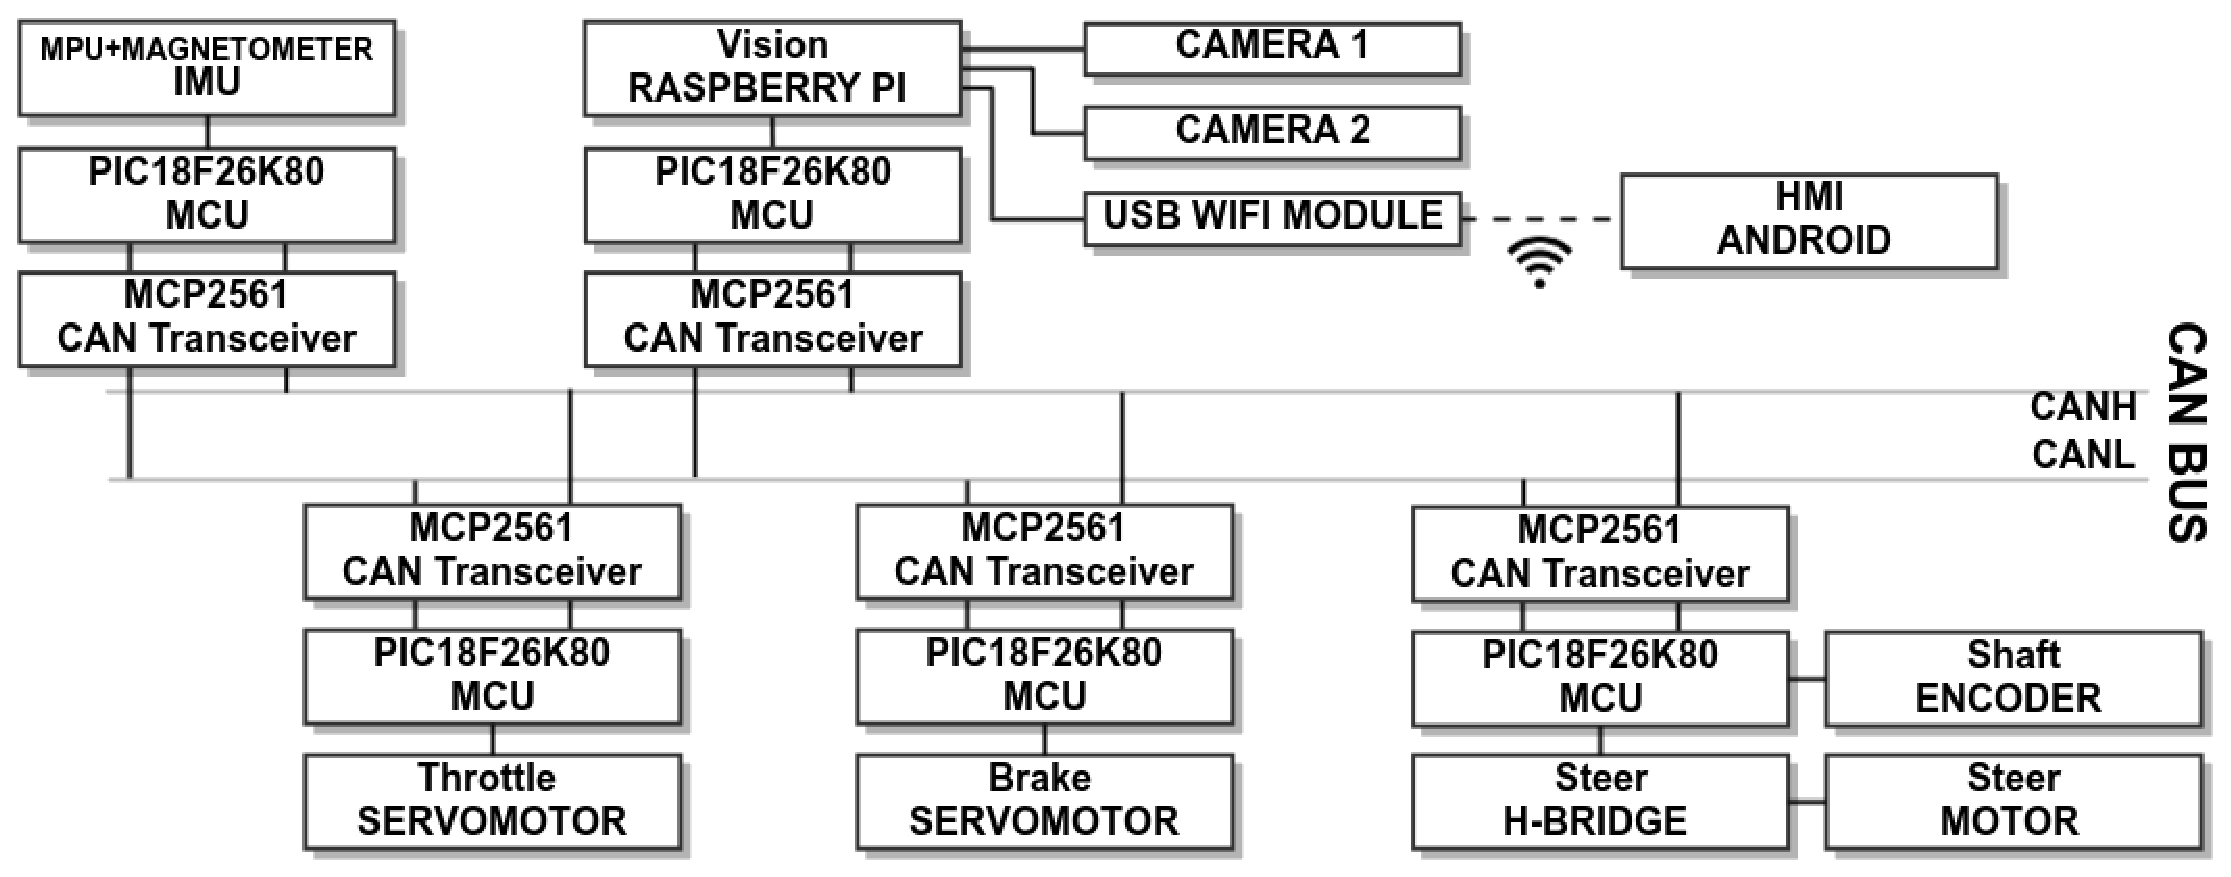
\includegraphics[height=5cm]{figs/fig_hw.eps}
\caption{Controller area network architecture}
\label{figs/fig_hw}
\end{center}
\end{figure*}

\begin{figure}
\begin{center}
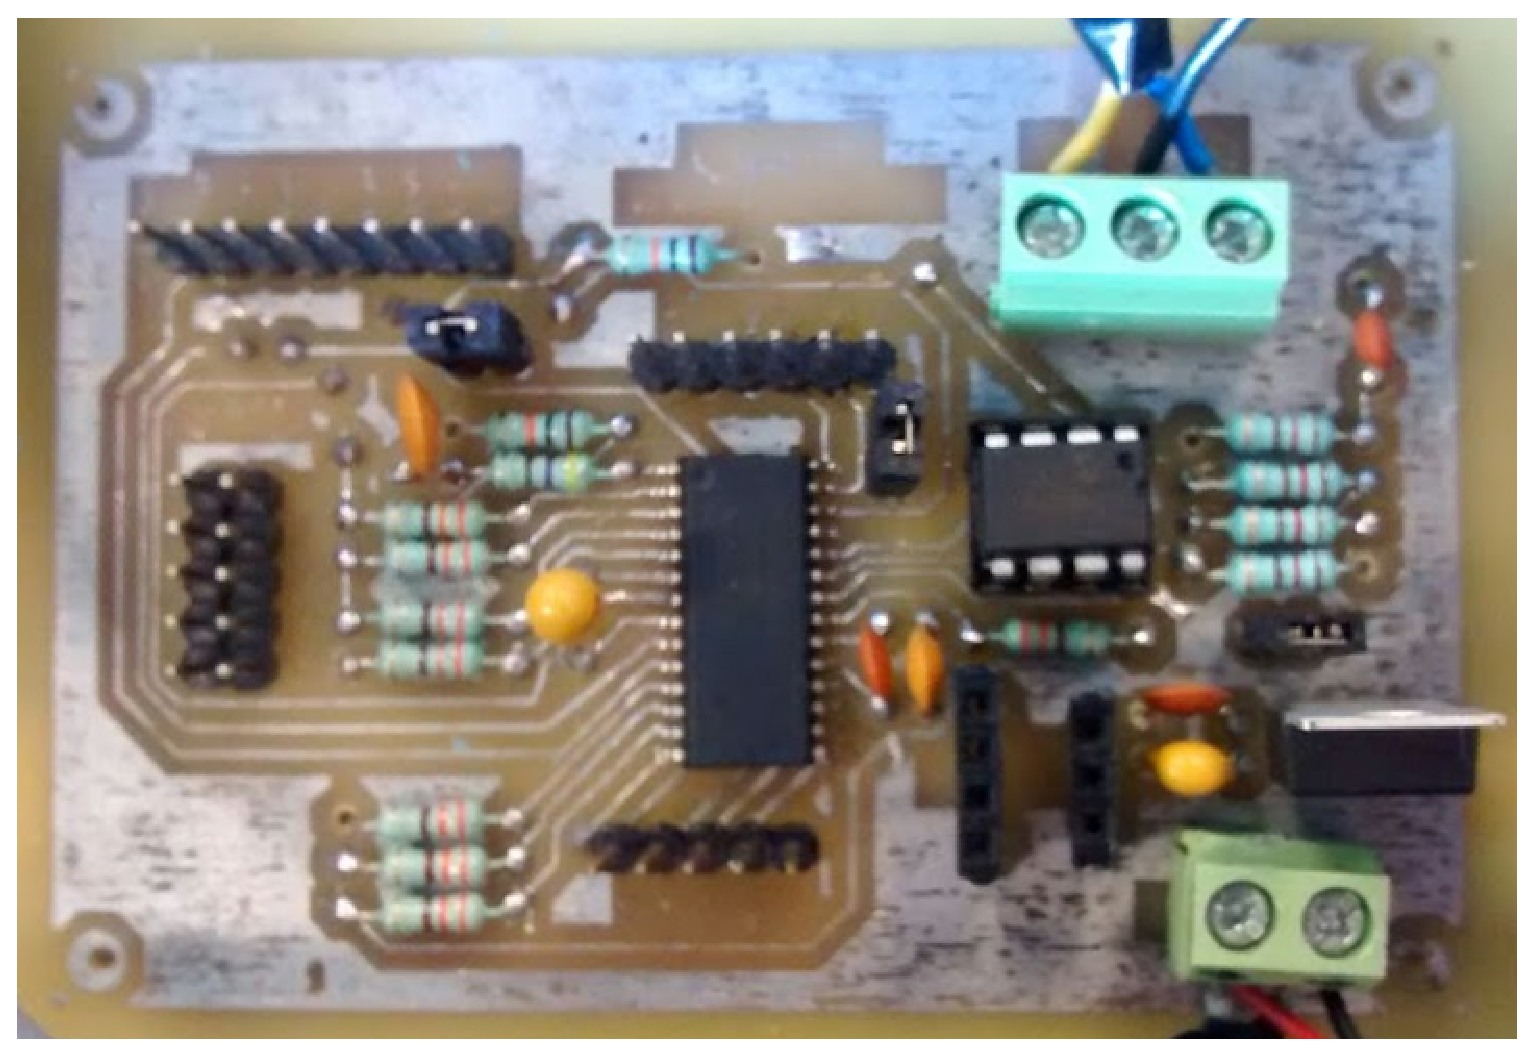
\includegraphics[height=3.8cm]{figs/fig_pcb.eps}
\caption{Generic sensor PCB designed (mainly) to interface sensors to the CAN bus}
\label{figs/fig_pcb}
\end{center}
\end{figure}

\subsection*{Steer-by-wire}
The most challenging system to interface to an electrical network was
the steering system. It consisted of a steering wheel used to turn a
shaft in contact with the rack and pinion that moved the bars which
pushed or pulled the wheels to the desired angle. Images of the steering
system are shown in figure~\ref{figs/fig_steer_photo}, drawings of
the assembly are shown in figure~\ref{figs/fig_steer}.

\begin{figure}
\begin{center}
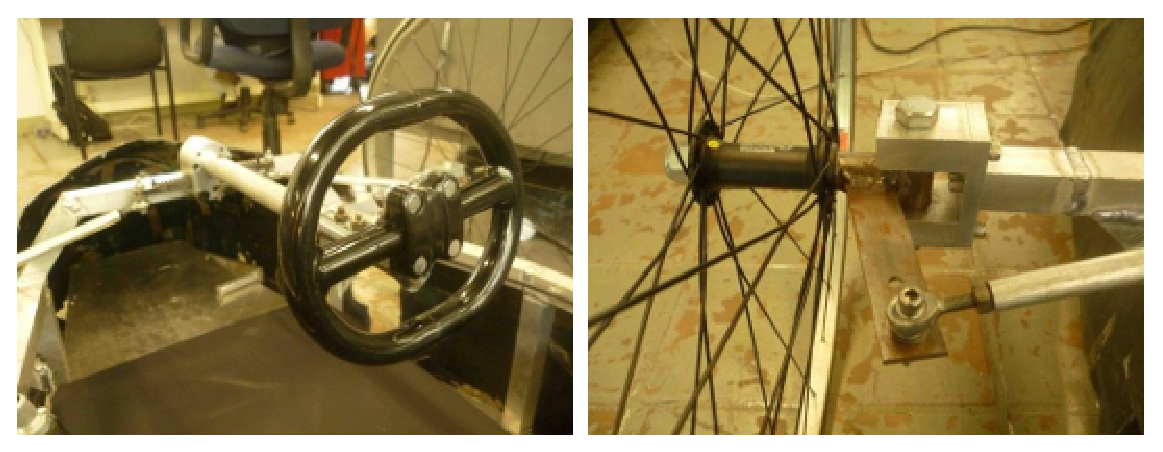
\includegraphics[width=8.1cm]{figs/fig_steer_photo.eps}
\caption{Picture of the assembled steering system}
\label{figs/fig_steer_photo}
\end{center}
\end{figure}

Figure~\ref{figs/fig_steer} shows the steering system is very simple.
If we consider it an assembly of a steering wheel, a steering shaft,
a cased bearing, a rack, joint bolts, bars and wheels it has only
eleven components. The steering shaft rotates approximately 320 degrees
from full-left to full-right state.

\begin{figure}
\begin{center}
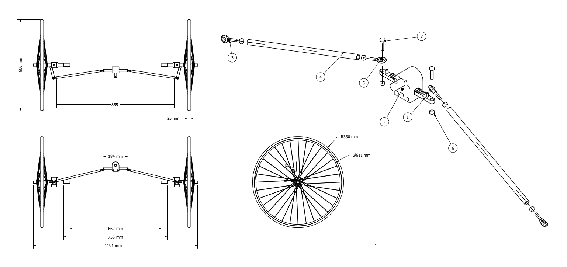
\includegraphics[width=8.1cm]{figs/fig_steer.eps}
\caption{Steering system assembly drawing}
\label{figs/fig_steer}
\end{center}
\end{figure}

\subsubsection*{Concept and parametrization.}
After evaluating different concepts and substantial modifications of
the mechanical system, the final approach was to consider the whole
current steering system as a blackbox driven by the steering wheel.
This approach allowed to measure the required torque and speed directly
on the existing system and to avoid doing unnecessary modifications
to the already very minimal mechanism.

A force sensor was mounted on the steering wheel (Fig.~\ref{figs/fig_steer_photo})
and measurements of the required force to turn the shaft were done on
different surfaces with a person on the car. The output of this measurements
was that the required force was 55N. The distance from the application point
to the axis of the shaft was 8cm therefore the needed torque was 4.4N$\cdot$m.
This is crucial information when choosing the actuators to be used on the
target machine. As mentioned before, for this case---few modifications, simple
transmission---measurements were straightforward and allowed to make a choice out of them.
If a big mechanical transmission had beeen replaced it would have involved more
considerations (such as the lost mass and friction).

Vehicle parametrization was done using the best available tool. If the
tool or infrastructure to do the measurement was not available data was
calculated/approximated. Mass and geometry-dependent parameters were
obtained using CAD software. Hardest-to-get parameters were approximated.
DivYX is a software developed at University of Monterrey that allows
computer aided kinematic analysis from a video registering frame by frame
the movement of a point of reference \cite{lperez}. Having these video-generated datasets
of how a system responds (its output) to different inputs allows to approximate
parameters that may otherwise be expensive to get---in time, money or complexity. Angular speed profiles
of the steering shaft for the very common double lane change, single lane
change and U-turn movements were also obtained using DivYX. This
is valuable information to feed into a simulation, to choose actuators/sensors
and to make decisions while implementing the controller.

\subsubsection*{The mechanism.}
Once the torque and speed needed were identified, a 12/24V DC motor (Table
\ref{motor_params}) was bought and a simple reduction mechanism was designed
and built. The blackbox approach put a very simple objective to the mechanism:
being able to generate the same movement an human could generate with the
steering wheel. To accomplish such objective---based on the information gathered
using DivYX---the mechanism had to produce an output speed of a 20th part of
the input (motor) speed and the output must be linked to the shaft where the
steering wheel used to be.

\begin{table}[ht!]
\centering
\begin{tabular}{ c | c | c }
\hline
Parameter & Value & Unit\\
\hline
Power & 0.17 & HP\\
Speed & 1800 & RPM\\
Torque & 5.84 & lb$\cdot$in\\
Voltage & 12/24 & V\\
Current & 16 & A\\
\hline
\end{tabular}
\caption{DC motor parameters}
\label{motor_params}
\end{table}

The desired reduction ratio could be obtained with two pairs of gears
and a pair of sprockets. The mechanism is shown in figure~\ref{figs/fig_gearbox}.
Spur gears, shafts, sprockets, a roller chain No. 40, bearings and retaining
rings are exposed and their positioning can be seen. Power rating and loads
capacities of transmission components were verified using manufacturer's tables.
The higher sprocket took the place of the steering wheel and the rest of the
mechanism (Fig.~\ref{figs/fig_steer}) was left untouched.

Actuation part is covered by the reduction mechanism and its motor, but any
closed-loop controller requires a form of feedback. In the case of a steering system a
shaft encoder is an usual choice. An absolute shaft encoder was mounted to the shaft and 
it was the final component needed to form an electromechanical interface from
an electronic controller to the steering system, allowing
manipulation of the steering motor to be done through an H-bridge using PWM
(Fig.~\ref{figs/fig_hw}). It is now a ``by-wire" mechanism.

\begin{figure}[ht!]
\begin{center}
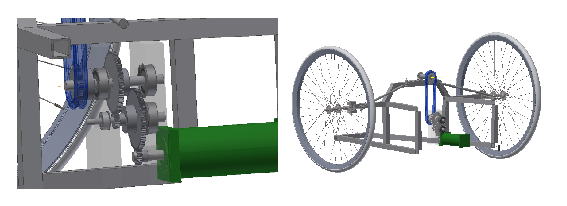
\includegraphics{figs/fig_gearbox.eps}
\caption{CAD model of the positioned reduction mechanism}
\label{figs/fig_gearbox}
\end{center}
\end{figure}

\subsection*{Brake-by-wire and throttle-by-wire}
These two systems were easier to implement due to their small force
requirements. The throttling pedal and its steel string were replaced
by a servomotor and another steel string. The braking lever and its
steel string were also replaced for a servomotor which was placed closer
to the V-brake. 

It was mentioned earlier that controllers require a form of feedback
but it is worth mentioning that at this development stage speed/acceleration
is not going to be autonomously controlled and, since the desired position
of a servomotor can be set using PWM, no extra sensors were added for
these systems. If feedback sensors were to be added options would include
odometers and tachometers, depending on the variable of interest.

%%%%%%%%%%%%%%%%%%%%%%%%%%%%%%%%%%%%%%%%%%%%%%%%%%%%%%%%%%%%%%%%%%%%%%
\section*{SIMULATION}

Cameras represented a challenge that was solved using a simulation platform.
Working on anything that needs to respond to space, geometry or 
color of its environment reduces the tools available. While it is possible
to simplify \cite{farooq}, break down or make assumptions about the problem
it is also possible to model all the features of interest to a ``virtual space"
\cite{Ryoichi}. Building a platform with a higher level of fidelity is an option that may or may not benefit
the project goals, thus it should be evaluated \cite{jayakumar}. 

Such platforms have many advantages that support overall development of a project.
They allow to work on the software when the real machine may not even exist
yet, to test multiple positioning of sensors without touching the real hardware,
to save testing time by running, aborting or restarting the simulation at any time,
faster than real time, for example.

While some projects may require a highly customized simulator, mature alternatives
that cover our sensors requirements and can be interfaced to external software exist.
These freely available simulators include V-REP, USARSim and Gazebo.
V-REP (Virtual Robot Experimentation Platform) is used in this project. It is
a piece of software used to simulate robots, their actuators, sensors and
the environments they interact with. Using V-REP saved plenty of time without sacrificing
the freedom to model the dynamics of the vehicle through a familiar interface (Simulink).

\subsection*{Dynamics Mathematical Model}
The models of the steer-by-wire with combined dynamics of the vehicle
chassis and the steering system from \cite{chang} were assembled in
Simulink. The states of the model are the chassis slip angle at the
center of gravity ($\beta$), the yaw rate ($\gamma$), the front steer angle ($\delta$)
and the front steer angle time derivative ($\dot{\delta}$). The chassis
slip angle is the angle between the direction of the displacement of the vehicle's
chassis and the direction it is pointing to. The yaw rate equals to how fast
the chassis is rotating around its yaw axis. The front steer angle is the angle
between the current direction of the wheel and its centered-position.
See figure \ref{figs/fig_chang} for the graphical description of these variables.

The mentioned states hold the information required to know the position and orientation
of the vehicle given an input to the DC motor of its steer-by-wire system. This model was
assembled using Simulink to be able to programmatically set the input current and read/visualize
the output. Assembled Simulink model is shown in figure~\ref{figs/fig_simulink}.
This figure shows the final Simulink file used to interact with the simulation. It is shown
input is read from and outputs are written to variables (these are labelled as $I\_M$, $B$, $G$, $D$ and
$DP$).

\begin{figure*}
\begin{center}
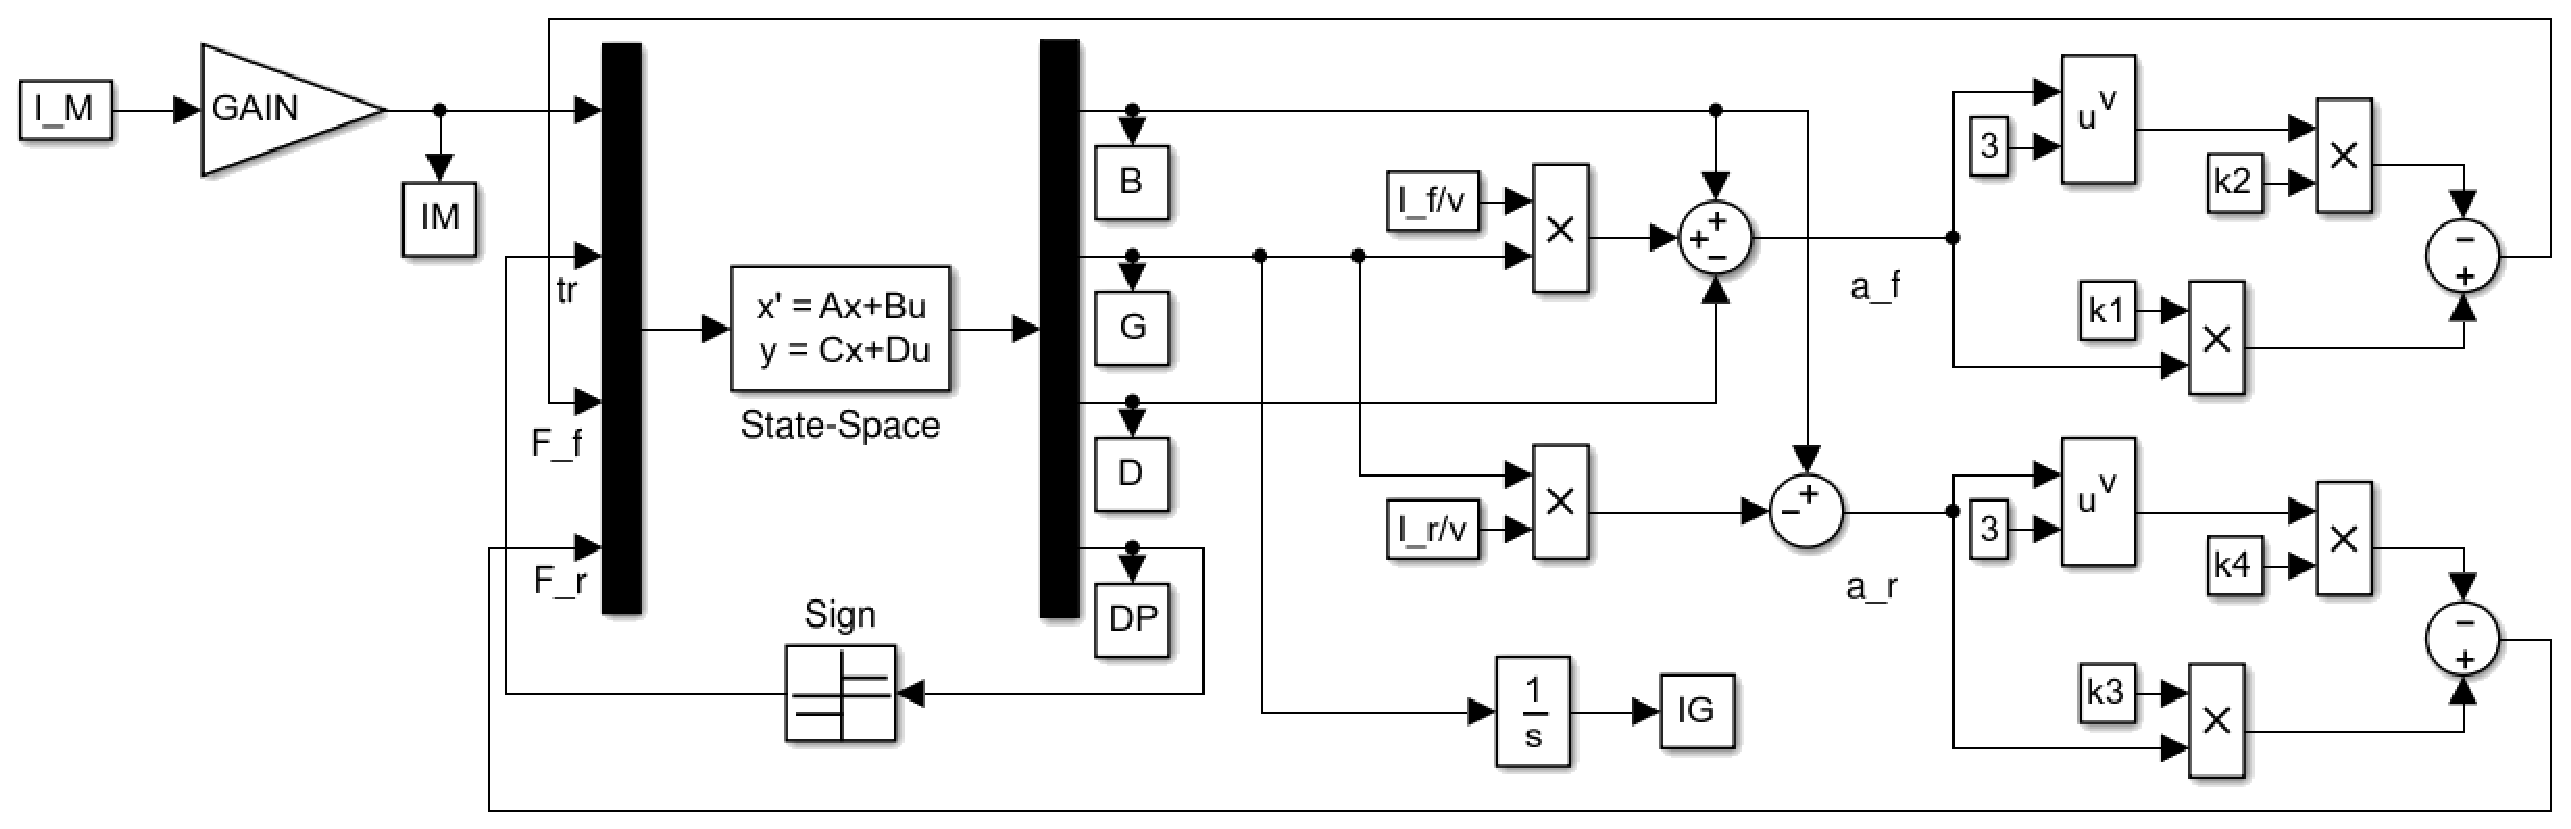
\includegraphics[width=14cm]{figs/fig_simulink.eps}
\caption{Simulink model for equations from \cite{chang}}
\label{figs/fig_simulink}
\end{center}
\end{figure*}

\begin{figure}
\begin{center}
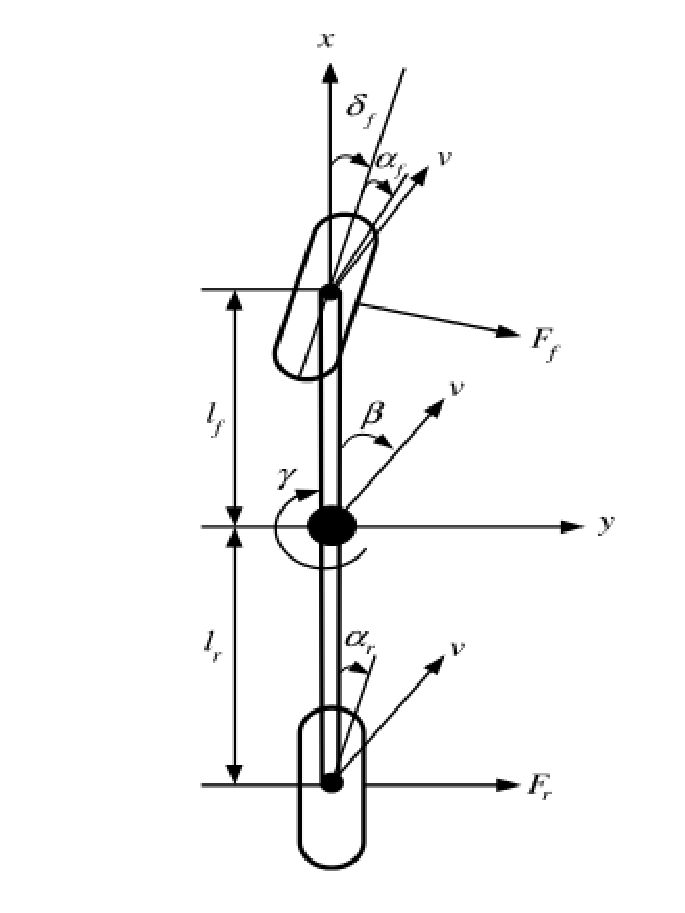
\includegraphics[height=6.8cm]{figs/fig_chang.eps}
\caption{Model of lateral motion of vehicle \cite{chang}}
\label{figs/fig_chang}
\end{center}
\end{figure}

%%%%%%%%%%%%%%%%%%%%%%%%%%%%%%%%%%%%%%%%%%%%%%%%%%%%%%%%%%%%%%%%%%%%%%
\subsection*{Virtual Platform}

While the final objective is to have an autonomous car that can drive
on a street and respond to external perturbations (such as people walking
into its way) the case study for this first step of the project (electrical
and mechanical instrumentation) is a simple line follower.

The platform consists of four main components. A diagram of the interactions between components is shown in figure \ref{figs/fig_platform}.
The platform was set up using: (0) a Matlab script for syncronization and interfacing of the components,
(1) Simulink for the simulation of the vehicle's dynamics, (2) V-REP for sensor
and environment simulation, (3) Probabilistic Hough Transform\cite{xuhough} C code
compiled using the MEX compiler is used for vision algorithms and a (4) MEX-compiled control algorithm
to compute the signal sent back to simulink. The goal of the platform is to simulate and evaluate
the computer vision and control algorithms.

Using Matlab to interface all the components provide a high-level entrance to
the platform. Its interaction with V-REP is done through V-REP Remote API---which allow
to control the modeled world from external software. Simulink models can be
started, paused, resumed and stopped from Matlab scripts. MEX-compiled C code can
also be called from Matlab scripts with little modifications to the original C source 
file---this ensures the same code will be able to run on the Raspberry used on the
real vehicle.

On the Simulink endpoint, after building and validating the equations for
steer-by-wire vehicle dynamics using blocks, the Simulink simulation is run
for a short period of time to calculate the direction in which the vehicle
will move, the rotation around its center of gravity and the angle of its
front wheels in response to a given current to the steering motor. This is crucial
information, because the information the cameras will capture depend on the
position and rotation calculated at this point.

V-REP was used to meet the requirement of simulating camera sensors mounted
on an input-responsive vehicle so the images of both cameras were
updated and feed back to the control block. The vehicles 3D CAD model was assembled,
the simulated cameras were mounted and a roadway modeled on V-REP (Fig.~\ref{figs/fig_vas_virtual}). The vehicle
3D model is positioned and rotated to the Simulink-computed state. Once the 
vehicle is at this new position new images are captured from its cameras.

Camera images are passed to the MEX-compiled Probabilistic Hough Transform 
program which is used for line-detection. This program discriminates from
the detected lines, selects the line the vehicle is following and returns
its angle. This angle is feed to a controller which returns the steering
motor current to the Matlab script and the whole process is run again.

\begin{figure}
\begin{center}
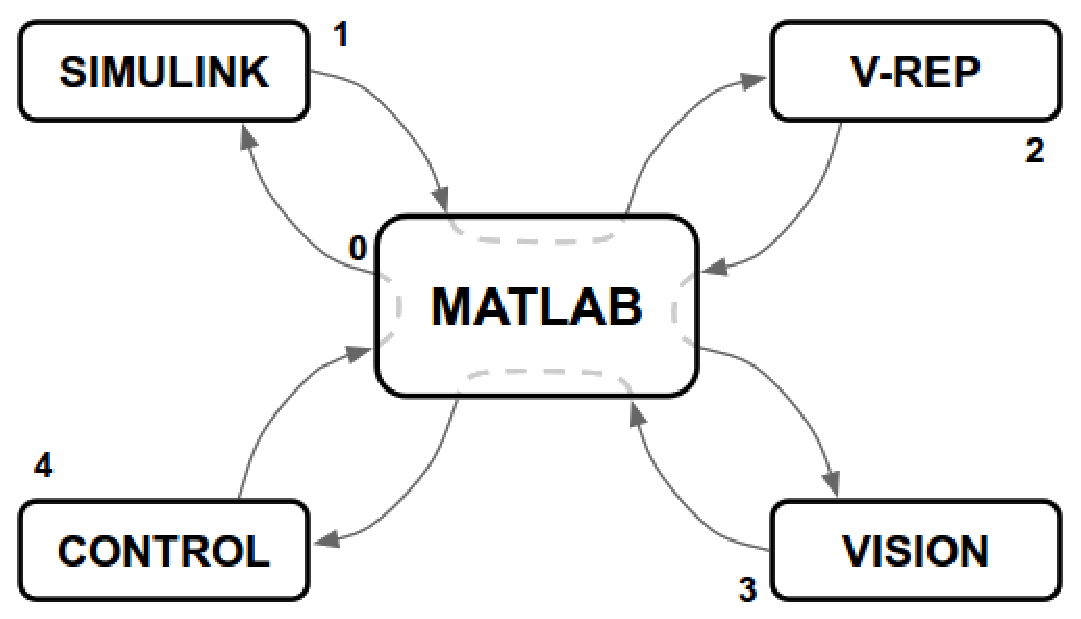
\includegraphics[width=6.5cm]{figs/fig_platform.eps}
\caption{Implemented Software-in-the-loop platform}
\label{figs/fig_platform}
\end{center}
\end{figure}

\begin{figure}
\begin{center}
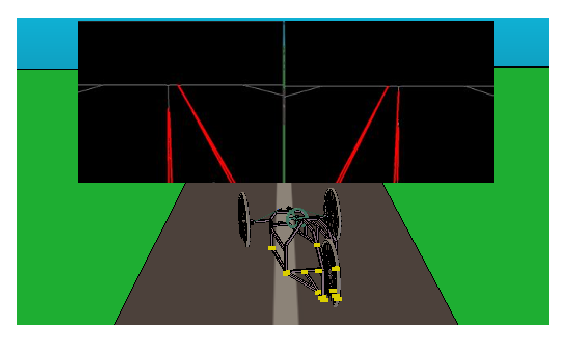
\includegraphics{figs/fig_vas_virtual.eps}
\caption{V-REP positioned model and line detection output}
\label{figs/fig_vas_virtual}
\end{center}
\end{figure}

\section*{RESULTS AND DISCUSSION}

\begin{figure}
\begin{center}
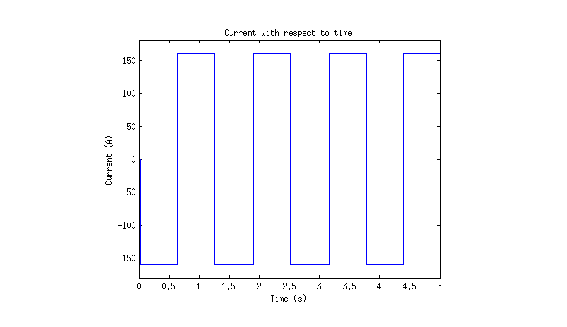
\includegraphics{figs/fig_ss_current.eps}
\caption{Amplified input current in amperes}
\label{figs/fig_ss_current}
\end{center}
\end{figure}

\begin{figure}
\begin{center}
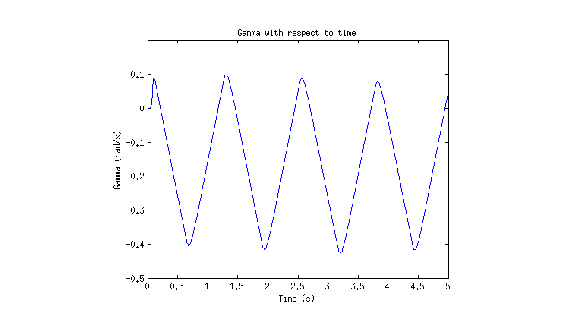
\includegraphics{figs/fig_ss_gamma.eps}
\caption{State variable $\gamma$ in rad/s}
\label{figs/fig_ss_gamma}
\end{center}
\end{figure}

\begin{figure}
\begin{center}
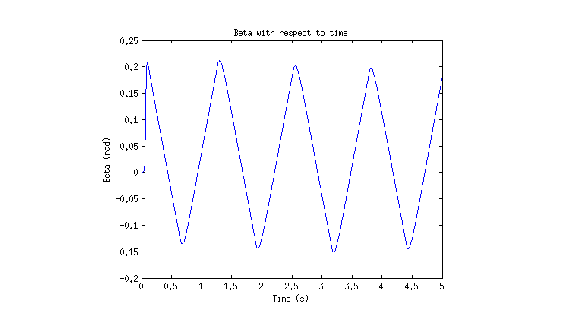
\includegraphics{figs/fig_ss_beta.eps}
\caption{State variable $\beta$ in rad}
\label{figs/fig_ss_beta}
\end{center}
\end{figure}

\subsection*{Virtual Platform}
The platform allowed to visualize the modeled vehicle dynamics on a 3D environment. Figure \ref{figs/fig_ss_current} shows the current inputted to the Simulink model to see the behavior of the vehicle on the simulation. Variation of the slip angle and yaw rate to such input is also shown (figures \ref{figs/fig_ss_gamma} and \ref{figs/fig_ss_beta}). Initial condition is with the steering at its centered position. The shown input current (Fig.~\ref{figs/fig_ss_current}) represents commanding the motor to alternate between running CW and CCW during equal intervals of time. Note that this should produce a movement which approximates to periodically turning a steering wheel with constant angular speed from center to left and back to center.

The expected yaw rate output is to see it increasing in magnitude while the current to the motor is being applied to the same direction, because this means the ``steering wheel" is being turned by the motor. At the same time the current starts flowing to the other direction the yaw rate should start to decrease in magnitude until it is around its initial condition of zero degrees (Fig.~\ref{figs/fig_ss_gamma}). The slip angle increases when turning to the left because the intertia of the vehicle will make it tend to go straight even if it has rotated.

This is the needed data to know what the cameras will capture from the next position of the vehicle. The other two states were only used for animation purposes. This data was sent to V-REP to reposition the 3D model of the vehicle within its environment. The result was the vehicle transiting the environment moving to the left following a zig zag path. This coherently matches with the current inputted to the dynamics model. What is being proposed here is the usage of V-REP as an extension of commonly used software (Matlab and Simulink) to use their mathematical models as the engine of 3D models in a V-REP environment which can be used to validate and take advantage of known dynamic models of machines to implement their required controllers.

This is a free alternative to also-available commercial software.

\subsection*{Real Vehicle}
The manufactured gearbox used on the steering system provided the expected (20:1) reduction ratio for the angular speed of the DC motor and allowed to smoothly turn the wheels using a PWM modulated signal on an H-Bridge. Figure \ref{figs/fig_picf_steer} shows the steering mechanism at the stage shown in figure \ref{figs/fig_gearbox}. Servomotors mounted to actuate the braking and throttling of the vehicle also allowed to manipulate these systems. Pictures of these actuators are shown in figures \ref{figs/fig_picf_brake} and \ref{figs/fig_picf_throttle}, respectively. 

Some boxes were mounted to protect the remaining electronic components and boards. Wires were also covered to protect them. These boxes and the instrumented vehicle in general are shown in figure~\ref{figs/fig_picf_vas}. Software that allowed to control the vehicle using an Android tablet connected through Wi-Fi was written to test the actuators were working properly. Implementation of different artificial intelligence and control methods will be discussed in another publication.

\begin{figure}
\begin{center}
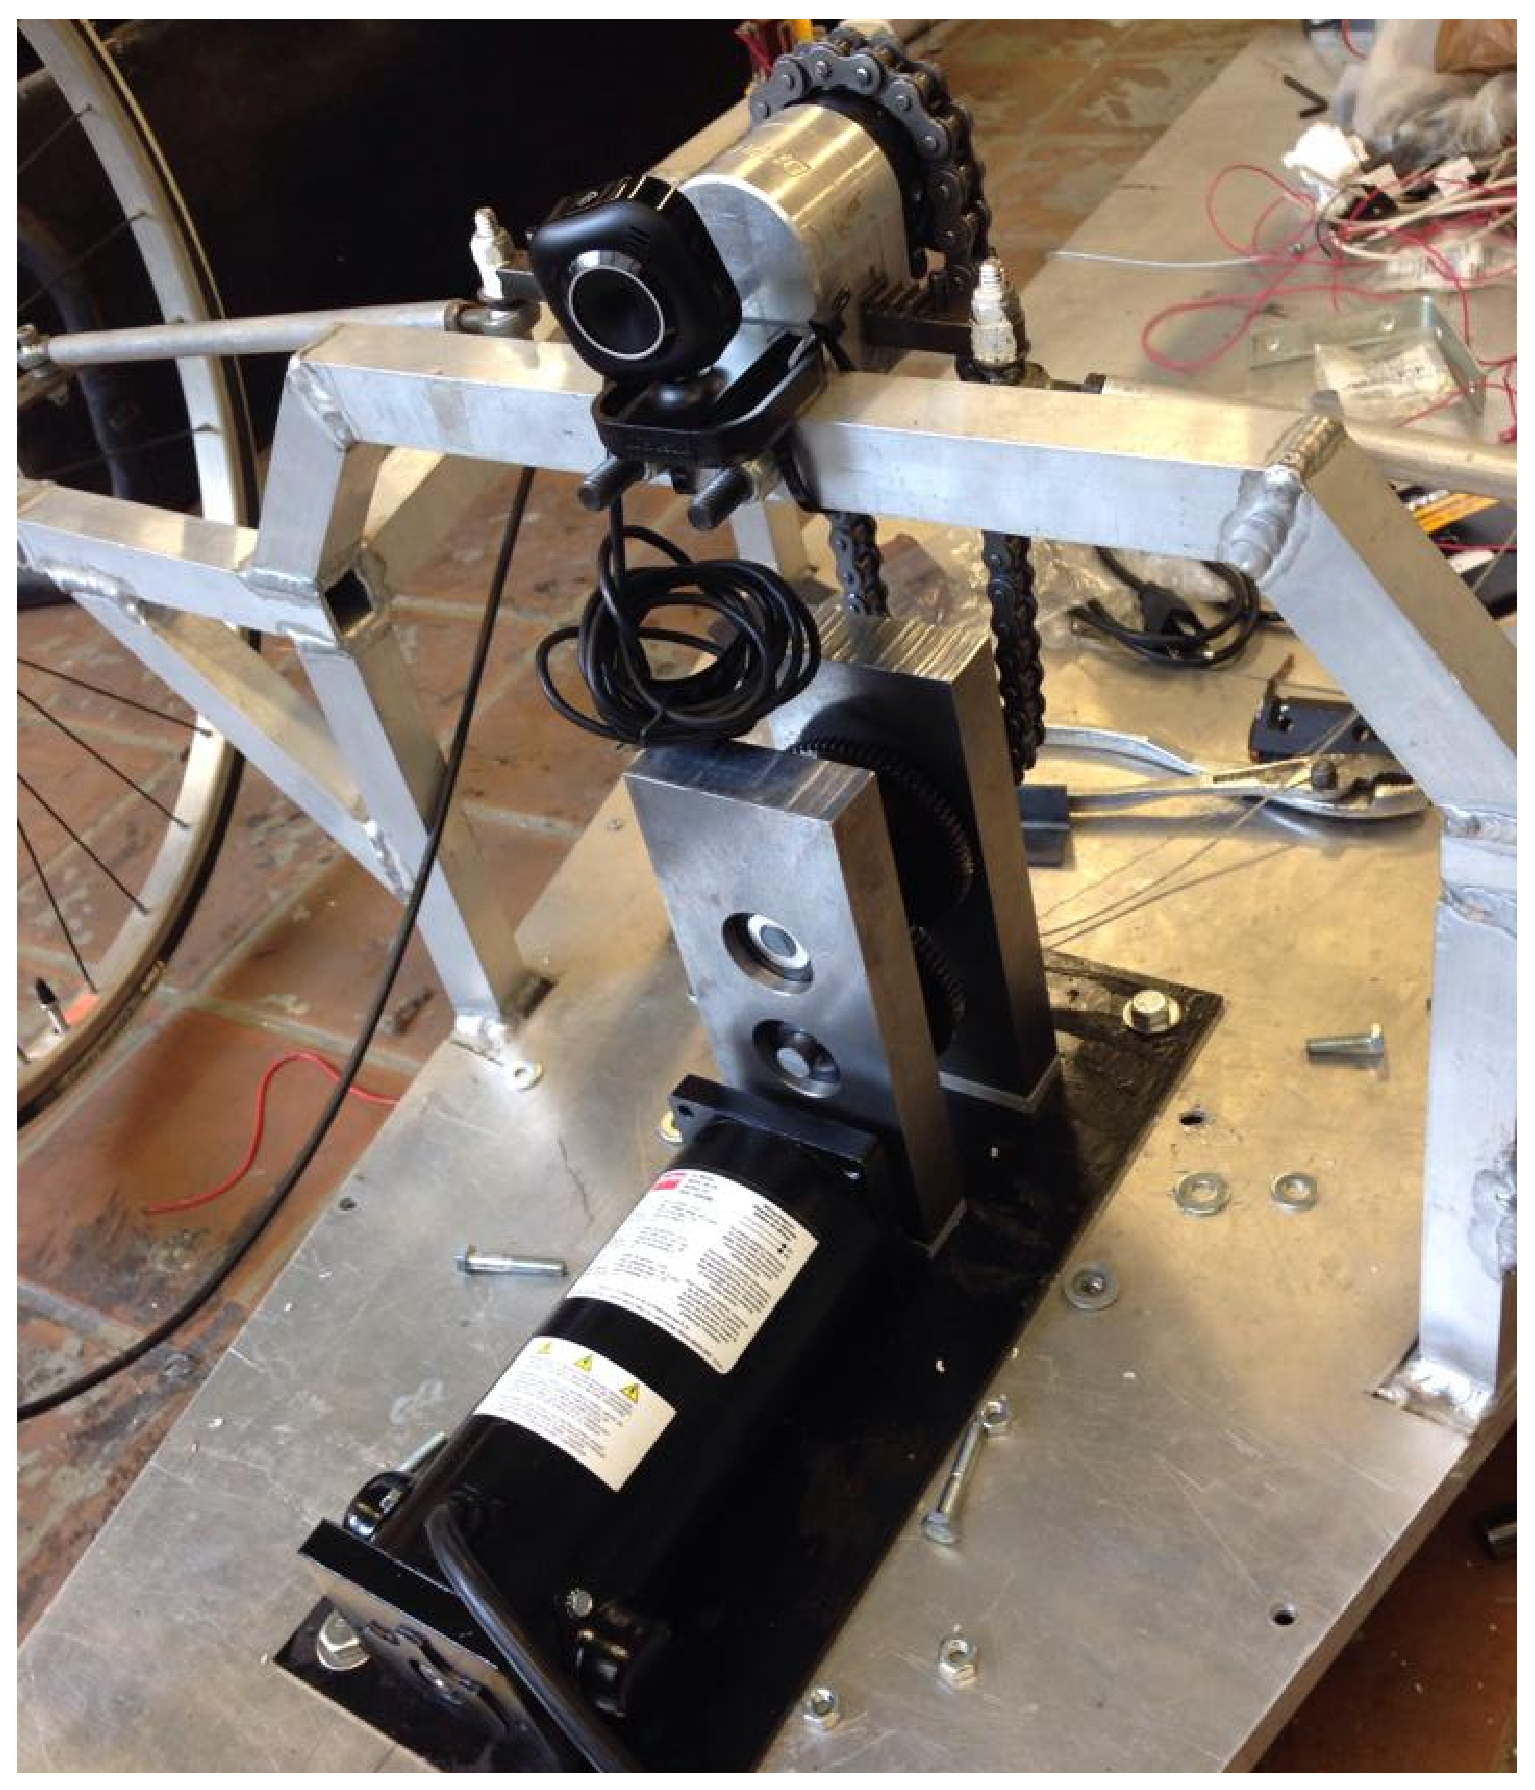
\includegraphics[width=5cm]{figs/fig_picf_steer.eps}
\caption{Uncovered steering reduction mechanism}
\label{figs/fig_picf_steer}
\end{center}
\end{figure}

\begin{figure}
\begin{center}
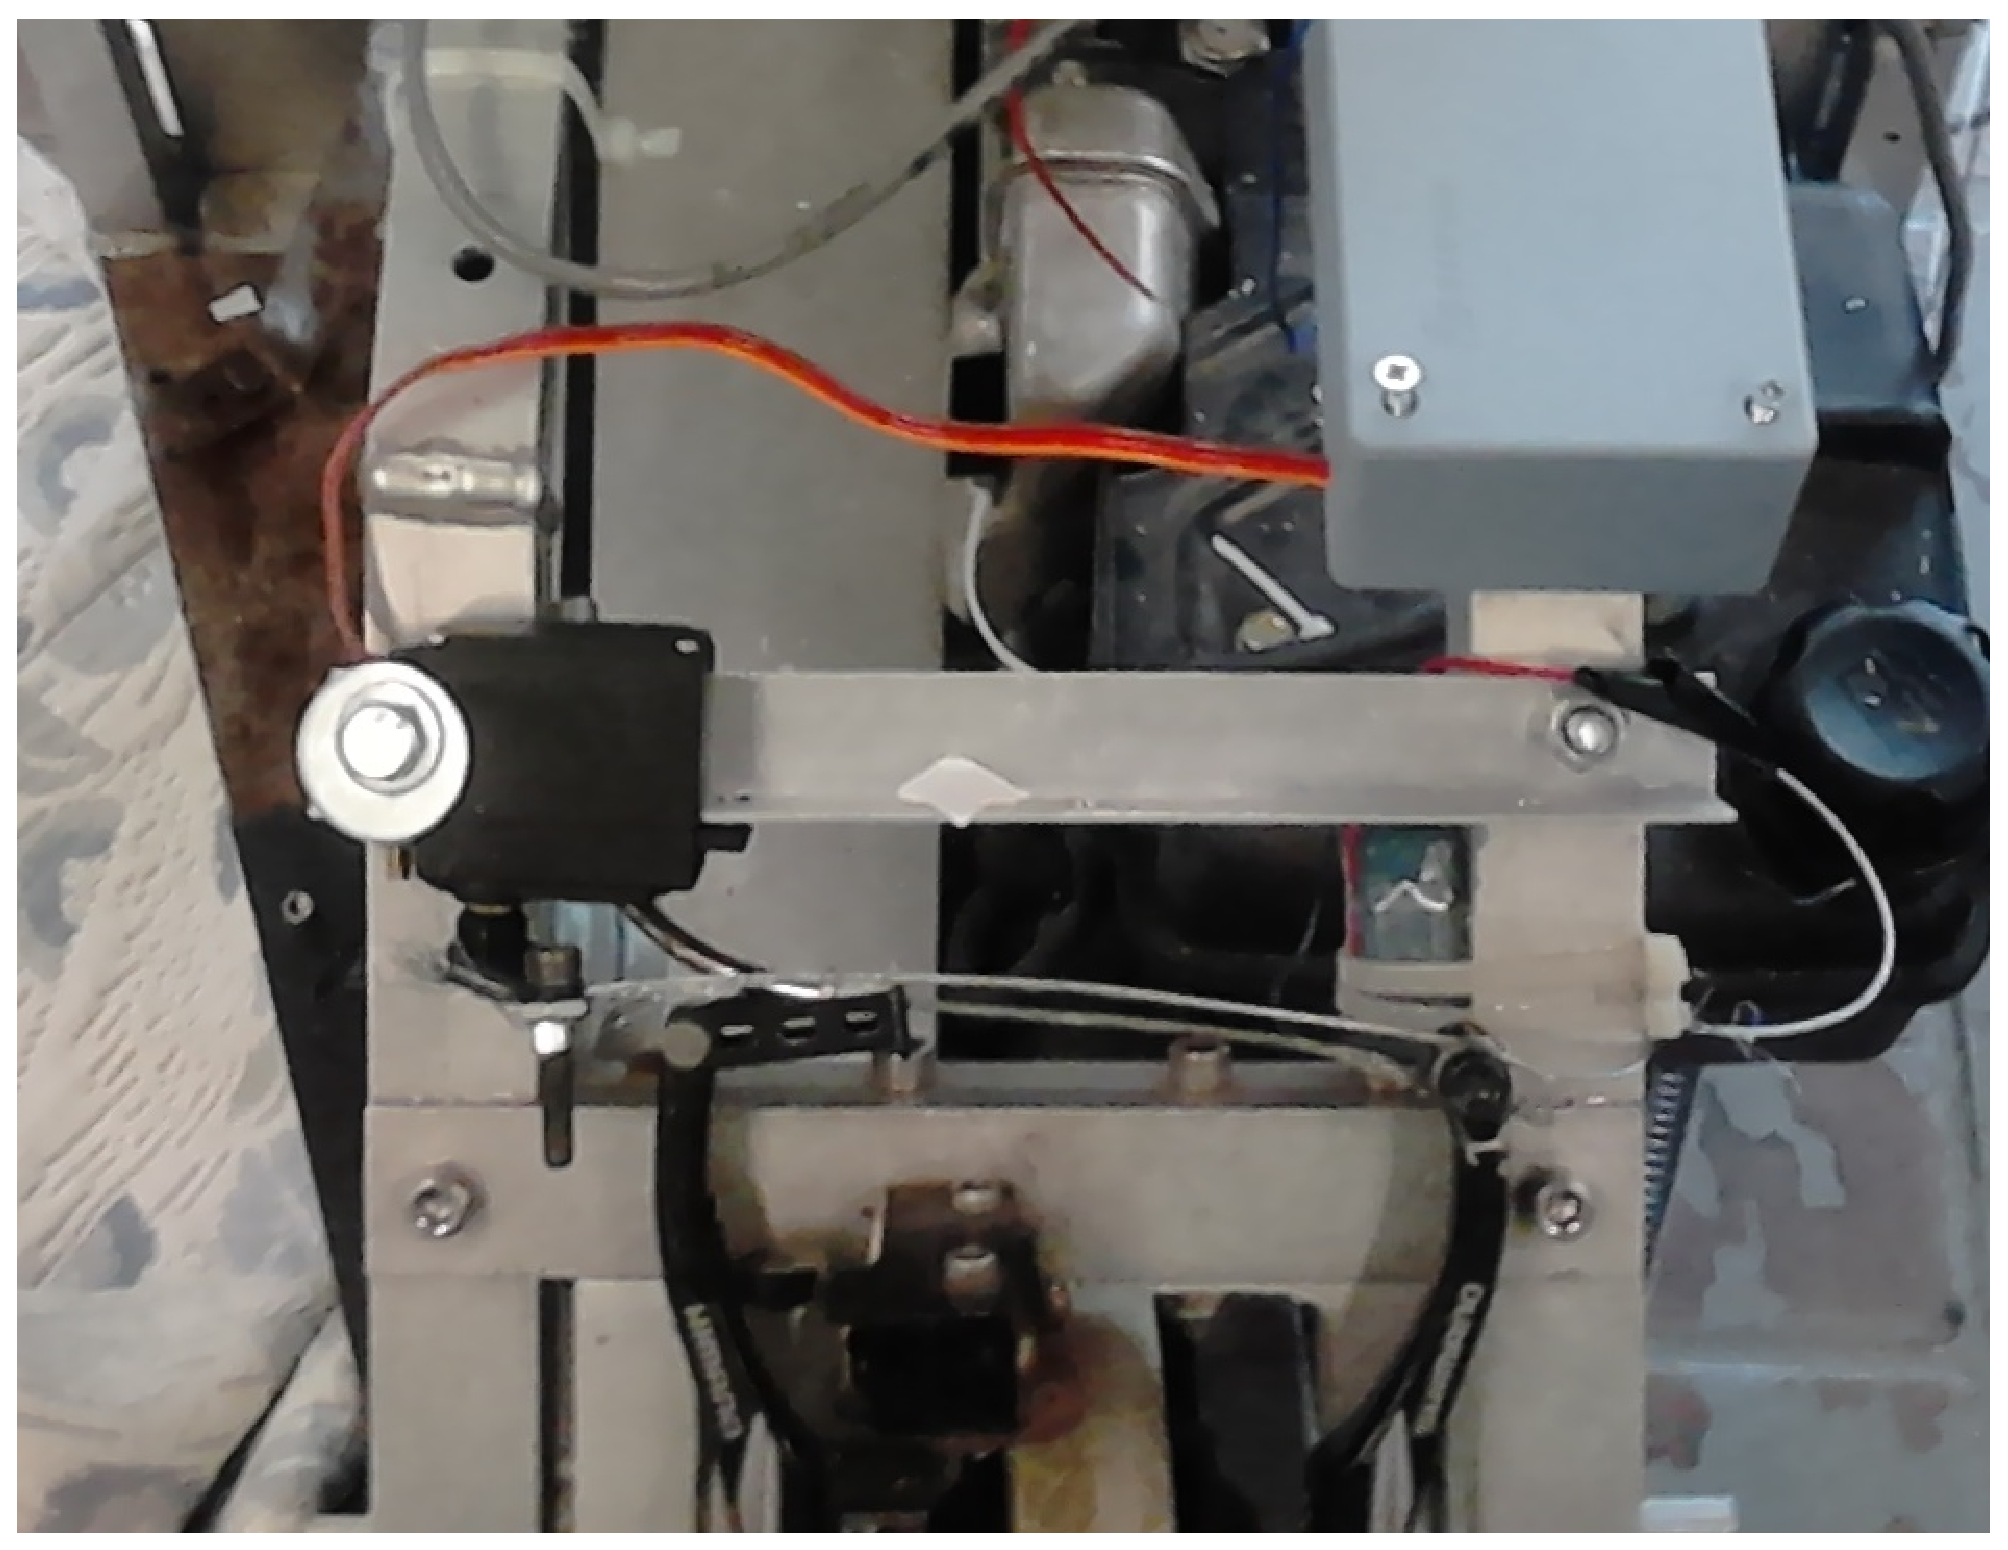
\includegraphics[width=7.5cm]{figs/fig_picf_brake.eps}
\caption{Servomotor mounted next to the V-brake}
\label{figs/fig_picf_brake}
\end{center}
\end{figure}

\begin{figure}
\begin{center}
\includegraphics[width=7.5cm]{figs/fig_picf_throttle.eps}
\caption{Throttle is actuated by this servomotor}
\label{figs/fig_picf_throttle}
\end{center}
\end{figure}

%%%%%%%%%%%%%%%%%%%%%%%%%%%%%%%%%%%%%%%%%%%%%%%%%%%%%%%%%%%%%%%%%%%%%%
\section*{CONCLUSION}

Building an autonomous machine is a multidisciplinary challenge. Mechanisms used within the machine must be mechanically reliable and allow the required movements. The use of electronics allow movement/force transmission to be done through wires instead of mechanical links. After completion of the electromechanical tasks, autonomous machines---a vehicle in this case---are excellent platforms to put to practice knowledge acquired from courses such as control engineering and artificial intelligence. The electromechanical tasks themselves also require knowledge from software, mechanical and electrical engineering.

General mechanical and electronic (software aside) procedure for converting a non-autonomous vehicle into an autonomous one was presented. This includes important aspects about the requirements of the underlying electronic architecture, interfacing a 3D simulator with software commonly used in engineering to deal with complex sensors (including but not limited to proximity, laser and cameras) and gathering information about the machine using kinematic video analysis. This insight to the path towards an autonomous vehicle can be of help when planning or taking design decisions on a similar project.

\begin{figure}
\begin{center}
\includegraphics[width=7.5cm]{figs/fig_picf_vas.eps}
\caption{Instrumented vehicle}
\label{figs/fig_picf_vas}
\end{center}
\end{figure}

\bibliographystyle{asmems4}
\bibliography{asme2e}

\end{document}
